% DO NOT COMPILE THIS FILE DIRECTLY!
% This is included by the other .tex files.

\begin{frame}
\titlepage
\end{frame}

\begin{frame}
  \frametitle{The aim of this presentation}
  \begin{itemize}
     \item A small update on the state of MISP's ongoing development
     \item Some highlights of the changes that were introduced
     \item Upcoming changes
     \item Cerebrate 1.0 and interactions with MISP
  \end{itemize}
\end{frame}

\begin{frame}
  \frametitle{MISP's evolution since the last MUG}
  \begin{itemize}
    \item Since the last MUG (02/09/2021) we've had:
    \begin{itemize}
        \item 2 releases with 1 additionally pending this week
        \item 920 commits
        \item 29 contributors contributing to the core software and its components
    \end{itemize}
  \end{itemize}
\end{frame}

\begin{frame}
  \frametitle{Heavy focus on the rework via Cerebrate}
  \begin{itemize}
      \item Refactoring parts of the code-base to prepare for the move
      \item Fixing several long standing issues
      \item Heavy focus also on integration
      \item Documentation of existing functionalities and mappings
  \end{itemize}
\end{frame}

\begin{frame}
  \frametitle{STIX libraries}
  \begin{itemize}
     \item Massive rework, the outcome of over a year of development by Christian Studer
     \item Added STIX 2.1 support on export
     \item STIX 1.1.1, 1.2, 2.0, 2.1 all supported
     \item Much more complex, in-depth mapping, aiming for 100\% coverage of the standard
     \item Collaboration with DHS and MITRE
     \item The MISP->STIX converters became their own standalone library
     \item Extensive documentation and examples for all possible generated objects
     \item Test suites to validate against MITRE's libraries
  \end{itemize}
\end{frame}

\begin{frame}
\frametitle{OpenAPI}
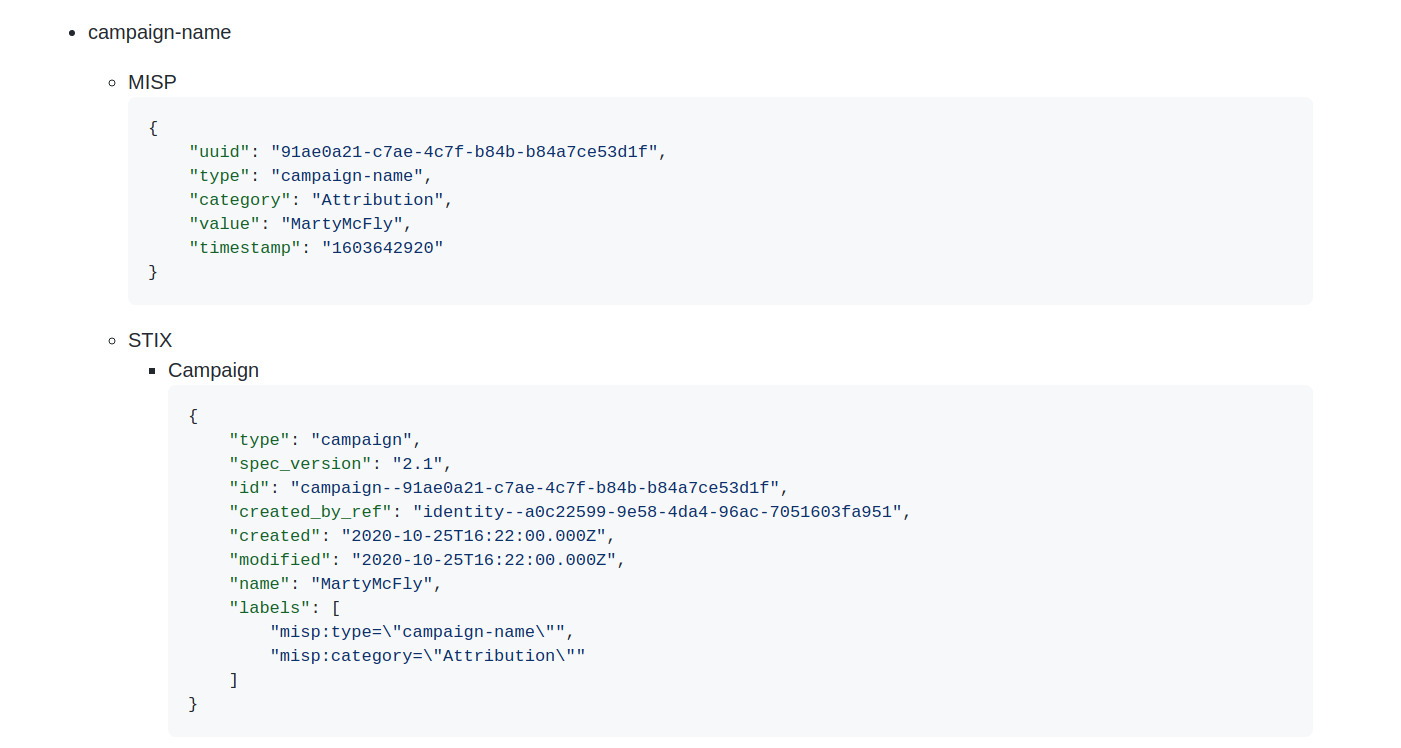
\includegraphics[scale=0.4]{images/stix.png}
\end{frame}

\begin{frame}
  \frametitle{Cerebrate integration rework}
  \begin{itemize}
     \item Connect MISP to Cerebrate
     \item Fetch organisation and sharing group information
     \item Update existing data with that of the Cerebrate repository
     \item For the reverse integration, we'll talk about where we are in the Cerebrate presentation
  \end{itemize}
\end{frame}

\begin{frame}
\frametitle{mail2misp 1.0 release}
\begin{itemize}
	\item A tool we've been using internally for a long time
        \item First official release
        \item Receive, parse, encode emails as MISP events
        \item Works with existing mail infrastructure or via a spamtrap
        \item Configure extensive parsing rules
\end{itemize}
\end{frame}

\begin{frame}
\frametitle{A host of improvements and fixes}
\begin{itemize}
	\item Massive amount o fxes, improvements to the core functionalities of the application
        \item Big thanks to Jakub Onderka for the constant stream of fixes
        \item Refactor of the internals to use the shared libraries with Cerebrate
        \item Move to a fork of the framework maintained by us
        \item Update of the certificate store that MISP uses by default
\end{itemize}
\end{frame}

\begin{frame}
\frametitle{New background processing library}
\begin{itemize}
	\item Finally, it is time to sunset the ancient background processor of MISP
        \item New tool, built from the ground up by Luciano Righetti
        \begin{itemize}
            \item More simplistic, relying on Supervisord
            \item No bloated scheduling - reliance on cron jobs
            \item Internally compatible with the old processor
        \end{itemize}
        \item For a period of time we will be supporting both concurrently
        \item Coming in MISP 2.4.151
\end{itemize}
\end{frame}

\begin{frame}
\frametitle{Supporting libraries}
\begin{itemize}
	\item Many updates to libraries such as:
        \item Taxonomies
        \item Galaxies
        \item Warninglists
\end{itemize}
\end{frame}

\begin{frame}
\frametitle{Integrations}
\begin{itemize}
	\item New MISP modules and improvements to existing ones
        \item Some examples:
        \begin{itemize}
            \item Integration with Alexandre Dulaunoy's newly developed Hashlookup service
            \item Passive SSH integration
            \item Recorded Future module
        \end{itemize}
\end{itemize}
\end{frame}

\begin{frame}
\frametitle{What's in the pipe?}
\begin{itemize}
	\item Further work on the move to the new tech stack
        \item Correlation engine rework
        \item Cryptographic {\bf signing of data}
        \item More flexible distribution model (multiple sharing groups)
        \item New UI
        \item Private Set Intersection (PSI) (allowing correlation sharing/privacy-aware export)
\end{itemize}
\end{frame}

\begin{frame}
\frametitle{Cerebrate}
\begin{itemize}
        \item Let's have a look at where we are at with Cerebrate
\end{itemize}
\end{frame}

\begin{frame}
  \frametitle{To sum it all up...}
  \begin{itemize}
     \item The MISP {\bf developer community} continues to grow and stay active
     \item The main focus this year is on the consolidation of existing functionalities
     \begin{itemize}
          \item Performance, security, UX improvements
          \item Monitoring and large scale management tooling
          \item Fleshing out the documentation and supporting materials
     \end{itemize}
     \item Cerebrate is aiming to fill the void of community/fleet management that we currently have
     \item Definitely no lack of new ideas and improvements, if you want to participate, it's easy to {\bf get involved}
     \item Prioritisation is hard. {\bf Let us know what you think we should focus on}!
  \end{itemize}
\end{frame}

\begin{frame}
  \frametitle{Get in touch if you have any questions}
  \begin{itemize}
    \item Contact CIRCL
    \begin{itemize}
      \item info@circl.lu
      \item \url{https://twitter.com/circl_lu}
      \item \url{https://www.circl.lu/}
    \end{itemize}
    \item Contact MISPProject 
    \begin{itemize}
      \item \url{https://github.com/MISP}
      \item \url{https://gitter.im/MISP/MISP}
      \item \url{https://twitter.com/MISPProject}
    \end{itemize}
    \item Cerebrate project
    \begin{itemize}
      \item \url{https://github.com/cerebrate-project}
      \item \url{https://github.com/cerebrate-project/cerebrate}
    \end{itemize}
    \item Join the COVID-19 MISP community
    \begin{itemize}
      \item \url{https://covid-19.iglocska.eu}
    \end{itemize}
  \end{itemize}
\end{frame}
